\documentclass[11pt,letterpaper]{article}
\usepackage[margin=.82in]{geometry}
\usepackage[T1]{fontenc}
\usepackage{lmodern,microtype,amsmath,amssymb,amsthm,graphicx,booktabs,xcolor}
\usepackage[colorlinks=true,linkcolor=blue!45!black,urlcolor=blue!45!black,citecolor=blue!45!black]{hyperref}
\setlength{\parindent}{0pt}
\setlength{\parskip}{6pt}
\newtheorem{theorem}{Theorem}
\title{\vspace{-1.5em}\textbf{Treating the Tremors We Built into Robots}\\[.4em]
\large A checked motion history, a tracking bound, and the cost of smoothing}
\author{Mike Helsel\\[-.2em]\small Working research note; AI assistance disclosed below}
\date{17 October 2026 \quad Draft for technical review}
\begin{document}
\maketitle
\vspace{-1em}
\begin{abstract}
Frequent target changes can produce unwanted motion even when each plan limits jerk. We study a scalar execution layer based on an established four-stage moving average. A Lean proof shows that its rational history check is equivalent to a bound on reference jerk at every future real time. A finite admission rule retains committed actions and preserves executed motion. A separate theorem connects this reference to a tracking bound for a stated uncertain actuator model.

A fixed comparison shows a benefit and a cost. The filter reduces motion in one hold task, but responds more slowly to a real target change. That hold input aligns with a frequency zero of the filter. A harder, predeclared comparison finds hold failures under irregular and random requests. A duration-limited baseline also removes much of the first apparent advantage. We distinguish formal proof, numerical evidence, and open implementation questions. This note does not claim a solution to general robot or VLA jitter.
\end{abstract}
\section{The problem is larger than smooth curves}
A planner requests a target. An execution layer turns requests into reference motion. A controller makes the machine follow that motion. These are different objects:
\[
\underbrace{g(t)}_{\text{task goal}}\qquad
\underbrace{q(t)}_{\text{reference position}}\qquad
\underbrace{x(t)}_{\text{physical position}}.
\]
Their errors satisfy
\begin{equation}\label{split}
x(t)-g(t)=[x(t)-q(t)]+[q(t)-g(t)].
\end{equation}
A small tracking error $x-q$ does not ensure a small task error $x-g$. The controller can accurately follow a reference that moves away from a stationary goal.

\textbf{Plain-language contract.} Keep motion already committed. Check the whole remaining reference before accepting a request. State the delay that the task can tolerate. Then bound the physical departure from that reference.

The artifact proves part of this contract for a finite scalar history. Requests have separate admission and execution times. The executor does not infer whether a small request is noise or a real change in intent. That distinction needs task information.

The title describes an engineering symptom. It does not imply a neurological mechanism or a common cause of all robot vibration. A coupled arm, contact, sampled control, and a learned policy remain outside this model.

\newpage
\section{An exact check of the retained reference}
Let $h>0$ be one moving-average width. Write $z_+=\max(z,0)$ and define
\[
F(z)=\frac{z_+^4-4(z-1)_+^4+6(z-2)_+^4-4(z-3)_+^4+(z-4)_+^4}{24}.
\]
This is the step response of four cascaded box averages. For a finite event list $E=((\tau_i,\delta_i))_{i=1}^n$, use
\[
q_E(t)=g_0+\sum_i\delta_i F\left(\frac{t-\tau_i}{h}\right),\qquad
j_E(t)=h^{-3}\sum_i\delta_i K\left(\frac{t-\tau_i}{h}\right).
\]
Here $K=F'''$ has branches $0,z,4-3z,3z-8,4-z,0$ on the consecutive intervals with boundaries $0,1,2,3,4$. Adjacent formulas agree at the shared boundaries. Lean proves the derivative chain through jerk at every point; $q_E$ is $C^3$.

At admission time $c$, form
\[
S(E,c)=\{c\}\cup\{\tau_i+kh:\ 1\leq i\leq n,\ k=0,\ldots,4,\ \tau_i+kh\geq c\}.
\]
\begin{theorem}[Finite check and future jerk]\label{guard}
For any finite list, $h>0$ and $J\geq0$,
\[
(\forall s\in S(E,c),\ |j_E(s)|\leq J)
\quad\Longleftrightarrow\quad
(\forall t\geq c,\ |j_E(t)|\leq J).
\]
For rational inputs, the executable Lean Boolean check is equivalent to this property over all real future times.
\end{theorem}
\textit{Proof idea.} Between consecutive roots, jerk is affine. Its absolute value is bounded by its endpoint values. After the last root, jerk is zero. The formal proof constructs the intervals from the event list. It covers an admission time between roots, repeated roots, empty histories, old events, and future events. Signed cancellation remains part of the check.

\textbf{Admission rule.} For admission time $c$ and execution time $\tau$, require $0\leq c\leq\tau$, nondecreasing admission times, and $\tau$ no earlier than the last committed execution. Express the new increment relative to the final committed target. Append it only if the future check passes. Invalid timing, rejection, and a no-change request retain history.

Finite induction proves the reference-jerk bound from the empty history. New events contribute zero through their execution time. Thus later admissions preserve the executed position, velocity, acceleration, and jerk. After the last execution time plus $4h$, the reference reaches the final committed target at rest. This does not assert physical rest or completion of a rejected goal.

\textbf{Boundary.} The wrapper receives one selected packet. Upstream batch selection and duplicate-conflict handling are not proved. Caller timestamps are not a proof of a real clock. The history is finite; bounded storage, pruning, infinite streams, and measured execution deadlines remain open. Exactness certifies the Lean rational check, not the Python scripts, input parser, upstream scheduler, or native solver. For $n$ events, the direct check visits at most $5n+1$ points and sums $n$ contributions at each. No real-time execution cost is established.

\newpage
\section{What the physical tracking proof says}
The scalar plant is
\begin{equation}\label{plant}
\dot x=v,\qquad \dot v=a,\qquad \dot a=r(t)[u+w(t)-a].
\end{equation}
Here $u$ is an acceleration command, $w$ is an additive acceleration disturbance, and $r$ is an actuator response rate. Let $\sigma>0$, with $8\sigma\leq r(t)\leq12\sigma$ and $|w(t)|\leq W$.

Use direct feedback
\begin{equation}\label{feedback}
u=\ddot q-8\sigma^2e_x-6\sigma e_v-\tfrac12e_a+\frac{5}{48\sigma}j,
\end{equation}
where $e_x=x-q$, $e_v=v-\dot q$, and $e_a=a-\ddot q$. No additional command filter is part of this theorem. Define
\[
z_1=e_x,\quad z_2=e_x+\frac{e_v}{4\sigma},\quad
z_3=e_x+\frac{e_v}{2\sigma}+\frac{e_a}{16\sigma^2}.
\]
\begin{theorem}[Conditional tracking bound]\label{tracking}
Fix $H\geq0$, $R\geq0$, and $\sigma>0$. Let $q=q_E$ be the admitted reference above and $j=q_E'''$. Suppose the physical state is a classical trajectory of \eqref{plant}--\eqref{feedback}, continuous on $[0,H]$, with the stated rate and disturbance bounds at every time in $[0,H]$. Suppose $|z_i(0)|\leq R$, $|j(t)|\leq J$ for every $t\in[0,H]$, and
\begin{equation}\label{budget}
W+\frac{J}{48\sigma}\leq2\sigma^2R.
\end{equation}
Then every $t\in[0,H]$ satisfies
\[
|e_x(t)|\leq R,\qquad |e_v(t)|\leq8\sigma R,\qquad
|e_a(t)|\leq64\sigma^2R.
\]
\end{theorem}
The composition proof derives the reference derivatives and jerk premise from the admitted history. It applies the earlier scaled invariant-cube theorem to the physical dynamics. The physical state is not reset at reference events.

\textbf{Illustrative values.} Use $\sigma=10\ \mathrm{s}^{-1}$, $h=.2\ \mathrm{s}$, $J=7.5\ \mathrm{m/s^3}$, $W=.01\ \mathrm{m/s^2}$ and $R=.2\ \mathrm{mm}$. The budget is $.025625\leq.04\ \mathrm{m/s^2}$. The rate interval is $[80,120]\ \mathrm{s}^{-1}$. No robot identification supports these illustrative values.

The theorem bounds $x-q$. A task-position guarantee also needs a bound on $q-g$ in \eqref{split}. It does not prove physical jerk below $7.5\ \mathrm{m/s^3}$, physical stopping, or a requested deadline. It assumes a physical trajectory exists. Existence for arbitrary discontinuous uncertainty is not proved.

\textbf{Proof evidence.} Independent computational review rebuilt the 44-module local dependency closure and replayed nine modules with the separate Lean checker. The audit covered 106 package theorem statements and 554 inherited statements. They are not 660 research discoveries. Only the standard axioms \texttt{propext}, \texttt{Classical.choice}, and \texttt{Quot.sound} appeared. Four false variants were rejected. These checks support the formal statements, not the physical model's validity.

\newpage
\section{The first comparison: motion versus response time}
The first gate has 72 cases: three methods, four synthetic request streams, three constant actuator rates, and two constant disturbances. Each has 1 ms and .5 ms output traces. Raw target changes, native Ruckig replanning, and the guarded four-box reference share the physical feedback law and continuous physical state.

Ruckig uses $|\dot q|\leq.1\ \mathrm{m/s}$, $|\ddot q|\leq.5\ \mathrm{m/s^2}$ and $|j|\leq7.5\ \mathrm{m/s^3}$. The FIR uses $h=.2\ \mathrm{s}$. The general admission theorem checks jerk only; it does not certify every velocity or acceleration limit.

\begin{center}\small
\begin{tabular}{lrrr}
\toprule
Across six plant settings & Raw & Ruckig & Four-box\\
\midrule
Hold: peak $|x|$ (mm) & .123--.136 & .986--1.014 & .0334--.0460\\
Hold: sampled peak $|\dot a|$ ($\mathrm{m/s^3}$) & 136--209 & 8.07--11.81 & .0364--1.20\\
Step: absolute settling time (s) & .5035--.504 & .6895--.690 & .9635--.964\\
\bottomrule
\end{tabular}
\end{center}
Ranges use the saved .5 ms traces and event samples. Times start at simulation time zero. The step commits at $.22$ s. Settling means no later sampled violation of $|x-g|\leq.2$ mm, $|v|\leq.001$ m/s and $|a|\leq.02$ m/s$^2$. The step deadline is $1.5$ s and its horizon is $2$ s; hold uses $1.9$ s and $2.5$ s. The revised-goal stream uses $1.75$ s and $2.25$ s; late/stale uses $1.5$ s and $2$ s. There is no infinite-time claim.

\begin{center}
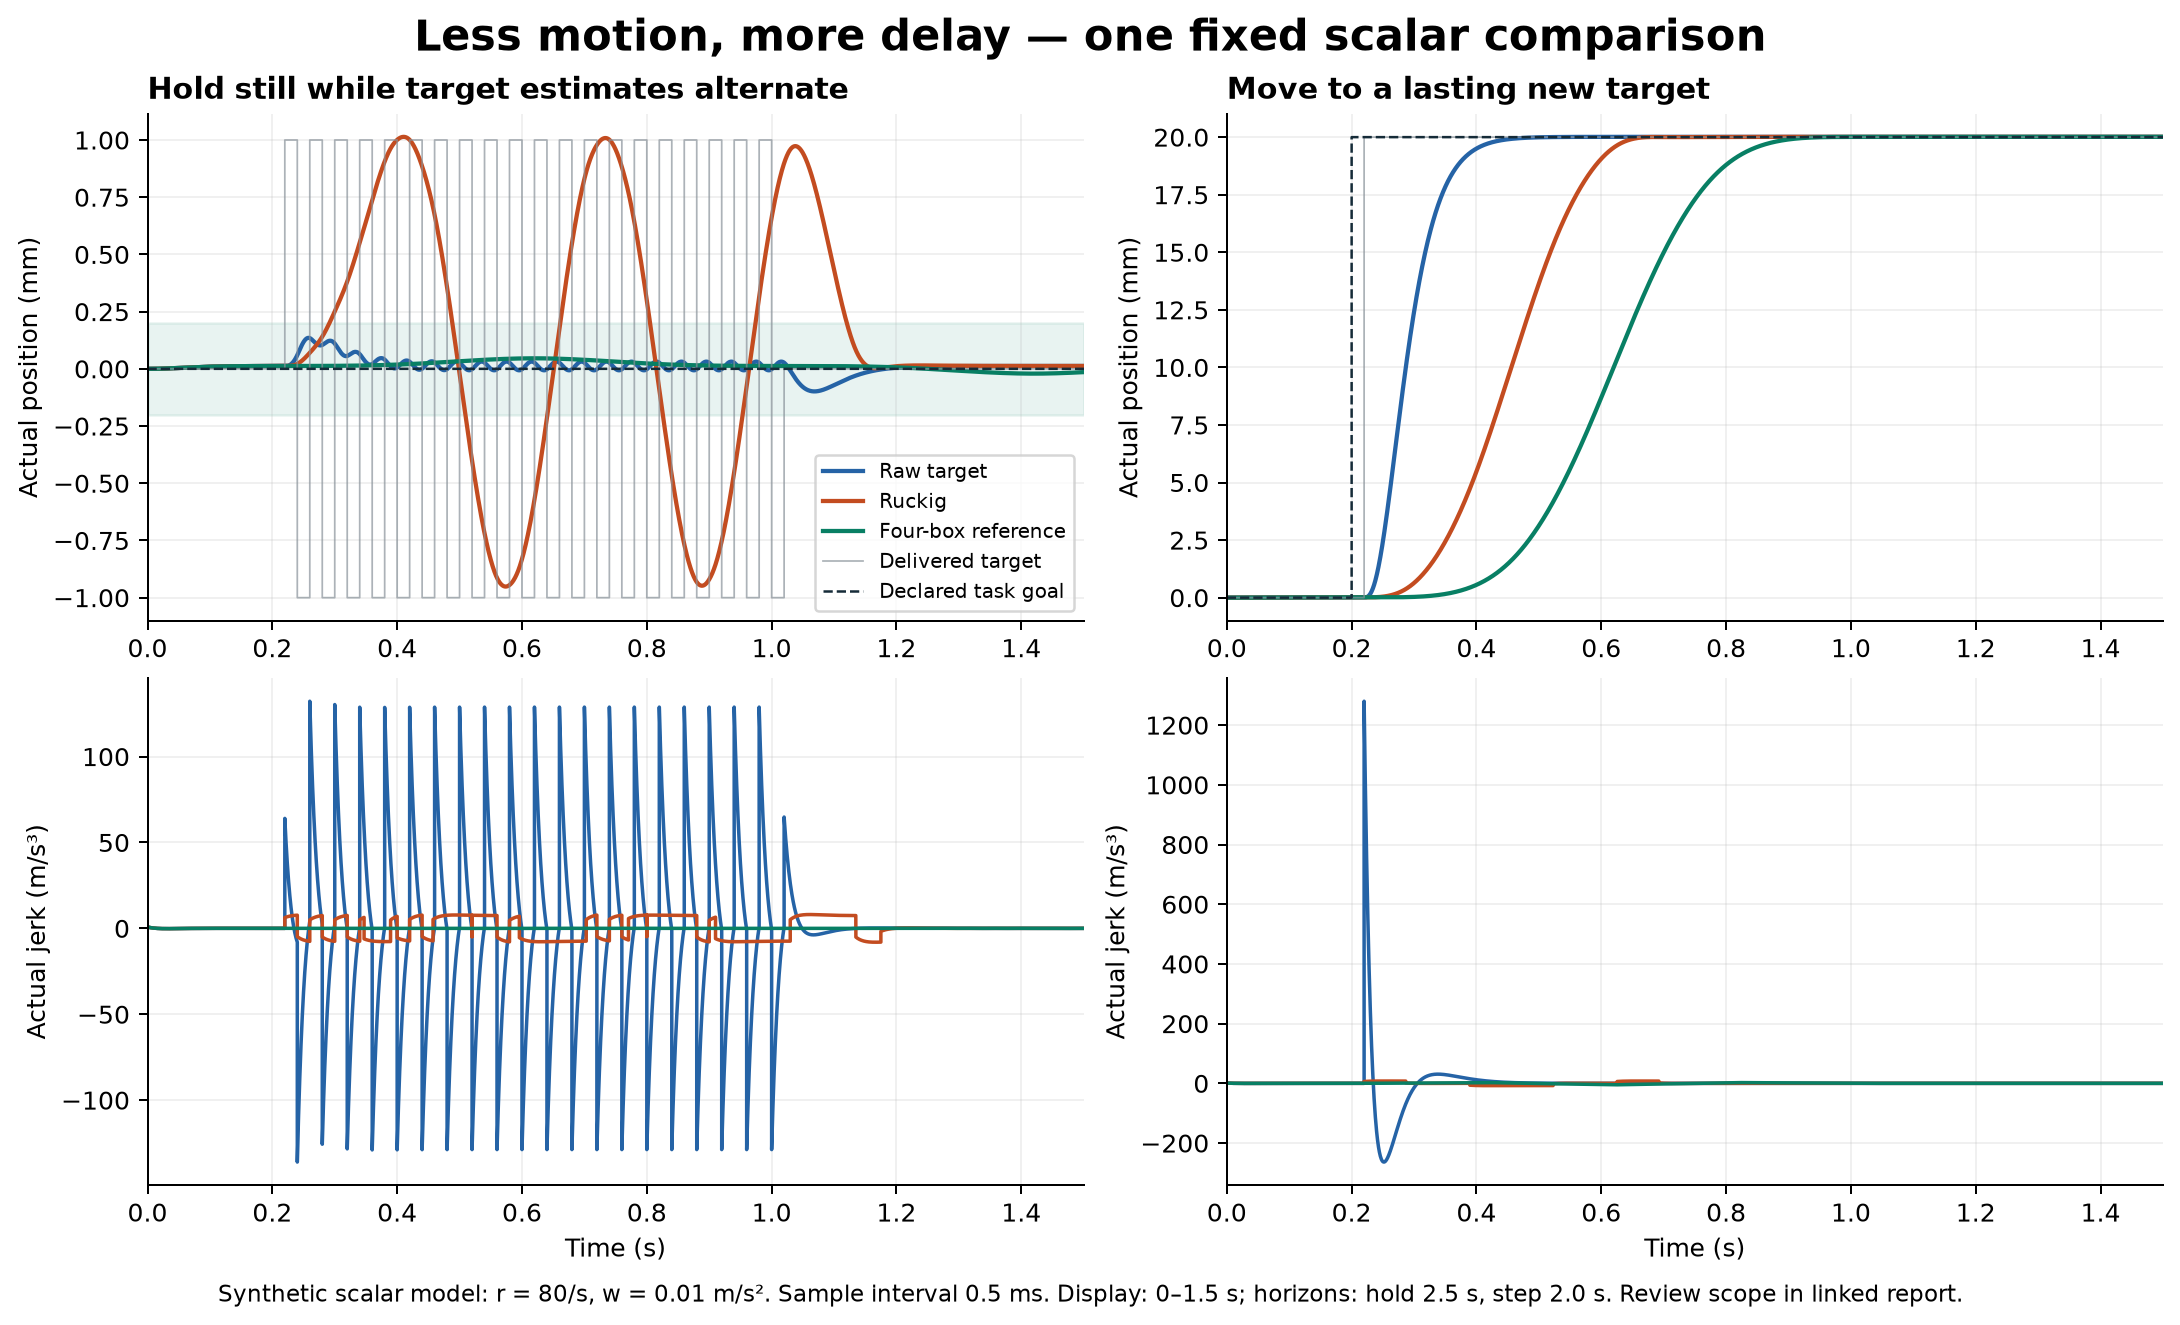
\includegraphics[width=\linewidth,height=3.45in,keepaspectratio]{images/comparison.png}
\end{center}
\vspace{-.8em}
{\small\textbf{Figure 1.} Fixed examples with $r=80\ \mathrm{s}^{-1}$ and $w=.01\ \mathrm{m/s^2}$. These curves and their peak metrics are numerical evidence.}

An independent 80-digit replay checked all 476,928 trace rows and 3,636 event rows. All 72 endpoint tests passed. Six Ruckig hold cases failed the added $.2$ mm hold band, leaving 66/72 full-task passes. All 24 FIR and 24 Ruckig cases passed the sampled position band $|x-q|\leq.2$ mm. This metric does not test the full transformed cube. The Lean history and composition certificate applies to FIR only. Ruckig has jerk switches and exported state roundoff; its passes are numerical. Raw steps also lie outside that proof contract.

\newpage
\section{The motion in the first hold example}
\begin{center}
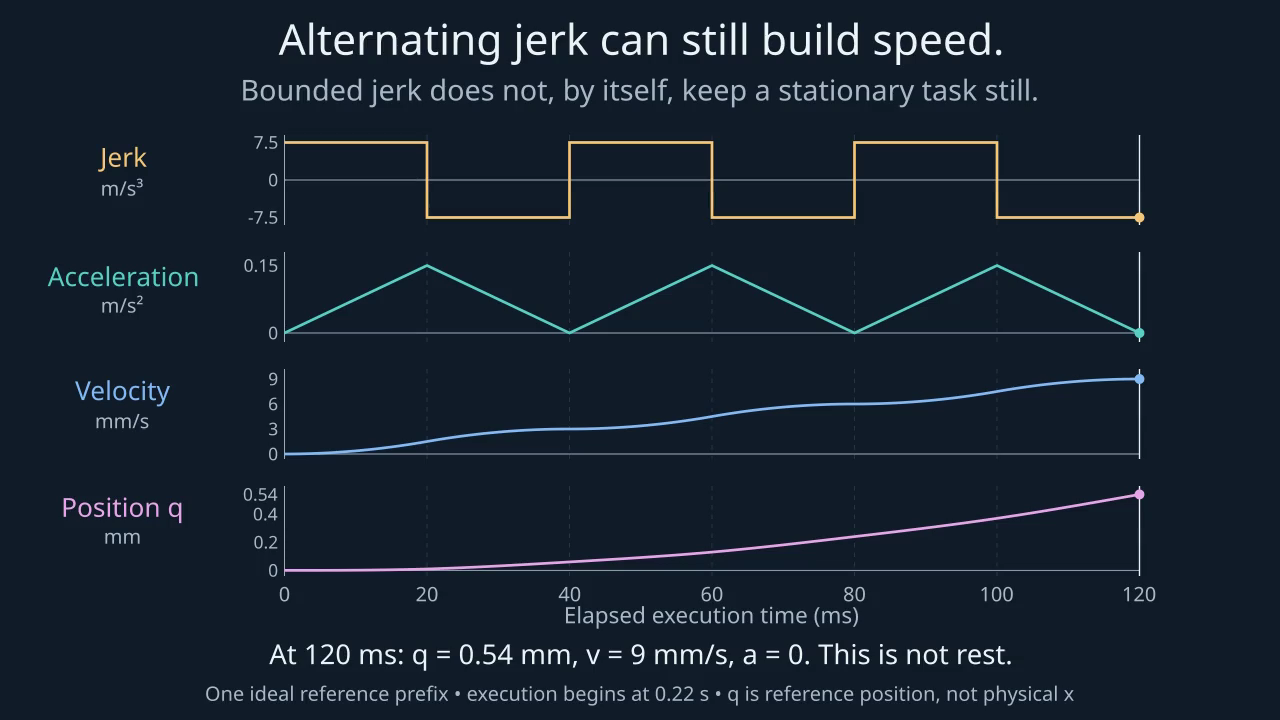
\includegraphics[width=\linewidth]{images/jerk-prefix-still.png}
\end{center}
\vspace{-.8em}
{\small\textbf{Figure 2.} Still from the accompanying Manim animation. It shows an ideal reference prefix, not physical axis motion. Exact segment endpoints match the independently reviewed native states within the recorded numerical tolerance.}

The first six executed intervals alternate jerk between $+7.5$ and $-7.5\ \mathrm{m/s^3}$. Each lasts 20 ms. Acceleration rises from zero to $.15\ \mathrm{m/s^2}$, then returns to zero. It stays nonnegative during this prefix, so velocity accumulates. After 120 ms, the reference has moved $.54$ mm and still has velocity $9$ mm/s.

This explains one trace without a clock error. Later replans change the pattern. It does not establish a defect in Ruckig, which solves a different local planning problem \cite{ruckig}. A bound on each plan's jerk does not by itself keep a stationary task still.

\textbf{The filter has a favorable input.} The target alternates every 20 ms. Its full period is 40 ms. One 200 ms box spans exactly five periods and cancels the sustained alternating signal after its start transient. Four boxes inherit that frequency zero. This example cannot establish general rejection of irregular jitter.

\textbf{The response is slower.} Four boxes have an 800 ms support and a 400 ms mean delay. In a retained negative case, a 20 mm step reaches only 10 mm by a deadline 400 ms after acceptance. A proposed 50 mm change fails the jerk check and is rejected.

\textbf{The guard does not cause these better curves.} Every primary FIR proposal passes. Removing the guard leaves the same reference. The guard rejects an invalid proposal and preserves committed history. Its proof and the filter's numerical performance are separate results.

\newpage
\section{A harder, predeclared comparison}
Gate 05 fixes six request streams and four methods before physical runs. It adds Ruckig with minimum duration $.8$ s at each replan. All 246 such plans return $.8$ s. This matches the FIR support, but does not ensure equal physical settling time.

The streams are the original periodic hold and step, 60 ms sign dwell (120 ms period), irregular alternation, seeded random targets, and biased targets. The four new streams have zero goal, a $3.5$ s deadline, and a $4$ s horizon. Requests, feedback, limits, three rates, and two disturbances are shared. Inputs and implementation were frozen before physical runs. Every FIR guard accepts; removing it leaves the same reference.

Independent 80-digit replay checked 144 cases at both output resolutions: 1,502,784 trace rows and 21,288 event rows. All 144 endpoint tests pass; only 66 full-task tests pass. All 108 smooth-method cases pass the sampled position band $|x-q|\leq.2$ mm, not a test of the full transformed cube. These are numerical results for the declared polynomial references, not additional Lean proofs.

\begin{center}\small
\begin{tabular}{lrrrr}
\toprule
Peak physical hold error (mm) & Raw & Fast Ruckig & Min. $.8$ s & FIR\\
\midrule
Periodic, 40 ms & .123--.136 & .986--1.014 & .034--.048 & .033--.046\\
60 ms sign dwell & .515--.544 & 1.000--1.020 & .075--.090 & .103--.115\\
Irregular & .796--.817 & .960--.997 & .178--.192 & .423--.435\\
Seeded random & .432--.445 & .891--.923 & .089--.102 & .234--.248\\
Biased & .411--.427 & .986--1.017 & .329--.342 & .400--.413\\
\bottomrule
\end{tabular}
\end{center}
Ranges use the $.5$ ms traces and event samples across six plant settings. The hold limit is $.2$ mm. The irregular stream has zero arithmetic mean but a time-weighted mean of $-.384615$ mm; unequal dwell times create bias. The random stream is one fixed realization, not a distribution-wide result. Every method fails the deliberately biased stream.

\textbf{A concrete filter failure.} With random targets, $r=80\ \mathrm{s}^{-1}$, $w=.01\ \mathrm{m/s^2}$ and $t=.896$ s, $x=.247558$ mm and $q=.234756$ mm. Tracking error is only $.012802$ mm, yet the hold band fails. The minimum-duration baseline passes. For the 20 mm step, settling after commitment is $.7975$--$.7980$ s for that baseline and $.7435$--$.7440$ s for FIR. FIR uses less jerk energy. No method wins every measure.

\textbf{The original execution check failed.} Two of 12 native checks have acceleration errors of $3.57\times10^{-9}$ and $7.42\times10^{-8}\ \mathrm{m/s^2}$, above the unchanged $10^{-10}$ limit. The second occurs on an ordinary grid point after repeated replans. The canonical path carries polynomial state at rational times; native execution carries its own state after double clock subtraction.

\textbf{A separate repair.} Gate 06 uses native retained state and binary execution origins, with unchanged inputs and limits. Independent preflight matches all 492 plans and 12 exported schedules. Independent 80-digit replay of 1,514,064 trace rows and 26,928 event rows reproduces unchanged task decisions. The finite native checks pass the original tolerances; they do not prove firmware fidelity. The old failed gate remains preserved.

\textbf{A metric can change while motion barely changes.} Total variation counts absolute changes, including jumps. For $\sigma=10\ \mathrm{s}^{-1}$ and SI units, a change at fixed physical state gives
\[
\Delta u=800\Delta q+60\Delta\dot q+1.5\Delta\ddot q+\Delta j/96.
\]
Two opposite $15\ \mathrm{m/s^3}$ jerk jumps add $5/16\ \mathrm{m/s^2}$ of command variation, even around a sub-picosecond phase. In biased fast Ruckig, ten such phases become five: jump variation changes by $-25/16\ \mathrm{m/s^2}$, with a state-join correction near $-1.65\times10^{-16}\ \mathrm{m/s^2}$. Continuous variation is separate. This exact audit does not establish a comparable motion change or sampled-actuator behavior.


\newpage
\section{Existing work and the remaining research claim}
FIR trajectory generation and derivative constraints are established. Biagiotti and Melchiorri study FIR planning and time optimization \cite{fir2012,fir2019}. Besset and B\'ear\'ee study online jerk-constrained FIR trajectories, including nonzero initial states and robot experiments \cite{fir2017}. Our four-box kernel is not a new smoothing method.

Real-Time Chunking retains committed actions while generating the remaining chunk \cite{rtc}. VLA-RAIL uses polynomial smoothing and chunk fusion with position, velocity, and acceleration continuity \cite{rail}. These close works prevent a broad claim to introduce a VLA smoothing layer. Our scalar experiment does not compare task performance against them.

Reference and command governors already use finite checks for future constraints, invariant fallbacks, and uncertainty bounds. The survey also treats asynchronous execution and plant-side acceptance \cite{governors}. ModelPlex derives checked arithmetic monitors from proved models and addresses bounded disturbances, clock drift, and arithmetic implementation \cite{modelplex}. These works rule out a broad claim to introduce future checking or a verified execution layer.

The narrower candidate is this list-parametric Lean rational guard, its retained-history contract, and its connection to a stated uncertain tracking bound. This is a specialized formalization and engineering case study. It is not yet an established new control method. The comparison ledger records which full methods were read and which FIR sources were only partly accessible. External specialist review is still needed to judge the artifact's research value.

\textbf{Limits on task intent.} If two tasks give the same observed history, a deterministic causal executor gives the same motion until the histories differ. If the tasks require goals $g_1$ and $g_2$, then
\[
|g_1-g_2|\leq |x-g_1|+|x-g_2|.
\]
At least one error is at least half the goal separation. This elementary argument is not a new theorem. It explains why a noise policy needs an intent or delay contract.

\textbf{Next publication gate.} Make the proof artifact easy to replay, preserve the negative cases, and seek human formal-methods and controls review before expanding the claim. A real action-stream test must report delay, task error, actual motion, and failures together. A scalar position request is not a full robot action chunk. Joint coupling, contact, sampled actuation, and task progress need further work.

{\small\raggedright\textbf{Reproducibility.} See \path{research/pods/2026-10-17/robot-motion/}: \path{certificate-03/}, \path{comparison-04/}, \path{latency-noise-05/}, \path{native-execution-06/}, and \path{jerk-prefix-animation/}. The proof bundle is in \path{publication/robot-motion/}, under \path{reviewer-bundle/}. Lean is version 4.35.0. The mathlib and Ruckig pins are:\par}
\begin{center}\small\ttfamily
56a005855ea17e0b0958f73ec801ae140b0a1679\\
99751e6ebc7c963bb80e99fbbe66f2c279d1db57
\end{center}
Ruckig cloud support is disabled.

Numerical replay treats exported floating coefficients as exact polynomial inputs and retains tiny positive phases. It is not bit-for-bit native execution. Switch-side differences remain in the reports. Physical states carry continuously from rest. Maxima and quadrature are numerical metrics.

\textbf{Contributions and assistance.} Mike Helsel set the question, proposed the execution-layer direction, identified the timing interpretation to test, and required fair comparisons and independent challenge. Codex agents assisted with sources, derivations, Lean proofs, numerical code, reviews, figures, and writing. Agent reviews are computational checks, not external human peer review. Author details, license, venue policy, and final claims remain to be settled before submission.

\newpage
\begin{thebibliography}{9}\small\raggedright
\bibitem{ruckig} L. Berscheid and T. Kr\"oger.
\emph{Jerk-limited Real-time Trajectory Generation with Arbitrary Target States}.
RSS, 2021. \url{https://arxiv.org/abs/2105.04830v2}.
\bibitem{fir2012} L. Biagiotti and C. Melchiorri.
\emph{FIR Filters for Online Trajectory Planning with Time- and Frequency-Domain Specifications}. Control Engineering Practice 20(12), 1385--1399, 2012.
\url{https://doi.org/10.1016/j.conengprac.2012.08.005}.
\bibitem{fir2017} P. Besset and R. B\'ear\'ee.
\emph{FIR filter-based online jerk-constrained trajectory generation}. Control Engineering Practice 66, 169--180, 2017.
\url{https://doi.org/10.1016/j.conengprac.2017.06.015}.
\bibitem{fir2019} L. Biagiotti and C. Melchiorri.
\emph{Trajectory generation via FIR filters: A procedure for time-optimization under kinematic and frequency constraints}. 2019.
\url{https://iris.unimore.it/handle/11380/1175126}.
\bibitem{rtc} K. Black, M. Y. Galliker, and S. Levine.
\emph{Real-Time Execution of Action Chunking Flow Policies}. NeurIPS, 2025.
\url{https://arxiv.org/abs/2506.07339v2}.
\bibitem{rail} Y. Zhao et al.
\emph{VLA-RAIL: A Real-Time Asynchronous Inference Linker for VLA Models and Robots}. 2025.
\url{https://arxiv.org/abs/2512.24673v1}.
\bibitem{governors} E. Garone, S. Di Cairano, and I. Kolmanovsky.
\emph{Reference and command governors for systems with constraints: A survey on theory and applications}.
Automatica 75, 306--328, 2017. \url{https://doi.org/10.1016/j.automatica.2016.08.013}.
\bibitem{modelplex} S. Mitsch and A. Platzer.
\emph{ModelPlex: Verified Runtime Validation of Verified Cyber-Physical System Models}.
Runtime Verification, 199--214, 2014.
\url{https://symbolaris.com/pub/modelplex.pdf}.
\end{thebibliography}
\end{document}
